	%!TEX root = ../../Main.tex
\graphicspath{{Chapters/Konklusion/}}
%-------------------------------------------------------------------------------


\section{Konklusion}

Der er i dette projekt blevet udviklet en prototype af en Bluetooth-baseret tyveri-alarm, af navnet BA-TA.
Prototypen kan gøre hverdagen nemmere for husets beboere, da man slipper for at have nøglen frem hver gang der skal låses eller låses op. Systemet har en godkendt liste af enheder, som systemet i Lock/lås auto state tjekker om er hjemme eller ej. Såfremt den ikke finder nogle af de godkendte enheder i nærheden bliver dørene i huset automatisk lås, som i denne prototype er grafisk implementer i hovedmenuen. Systemet er yderst brugervenligt og kan håndteres ved brugerinterakton igennem brugergrænsefladen.

Undervejs i projektet er der formået at omsætte den kendte teori og viden fra undervisningen, samt at hente ny information og viden fra forskellige kilder på internettet, datablade og lignende. 

En endelig udvikling og lancering af et produkt baseret på denne prototype vil dog kræve nogle modificeringer og tilføjelse af funktionalitet, som kan kategoriseres som fremtidigt arbejde.

Medlemmerne af projektgruppen er rigtig tilfredse med prototypen, dens samlede funktionalitet og test-resultater, og mener derfor at kravene til hhv. projektet og denne rapports omfang er opfyldt.

\begin{figure}[H]
	\centering
	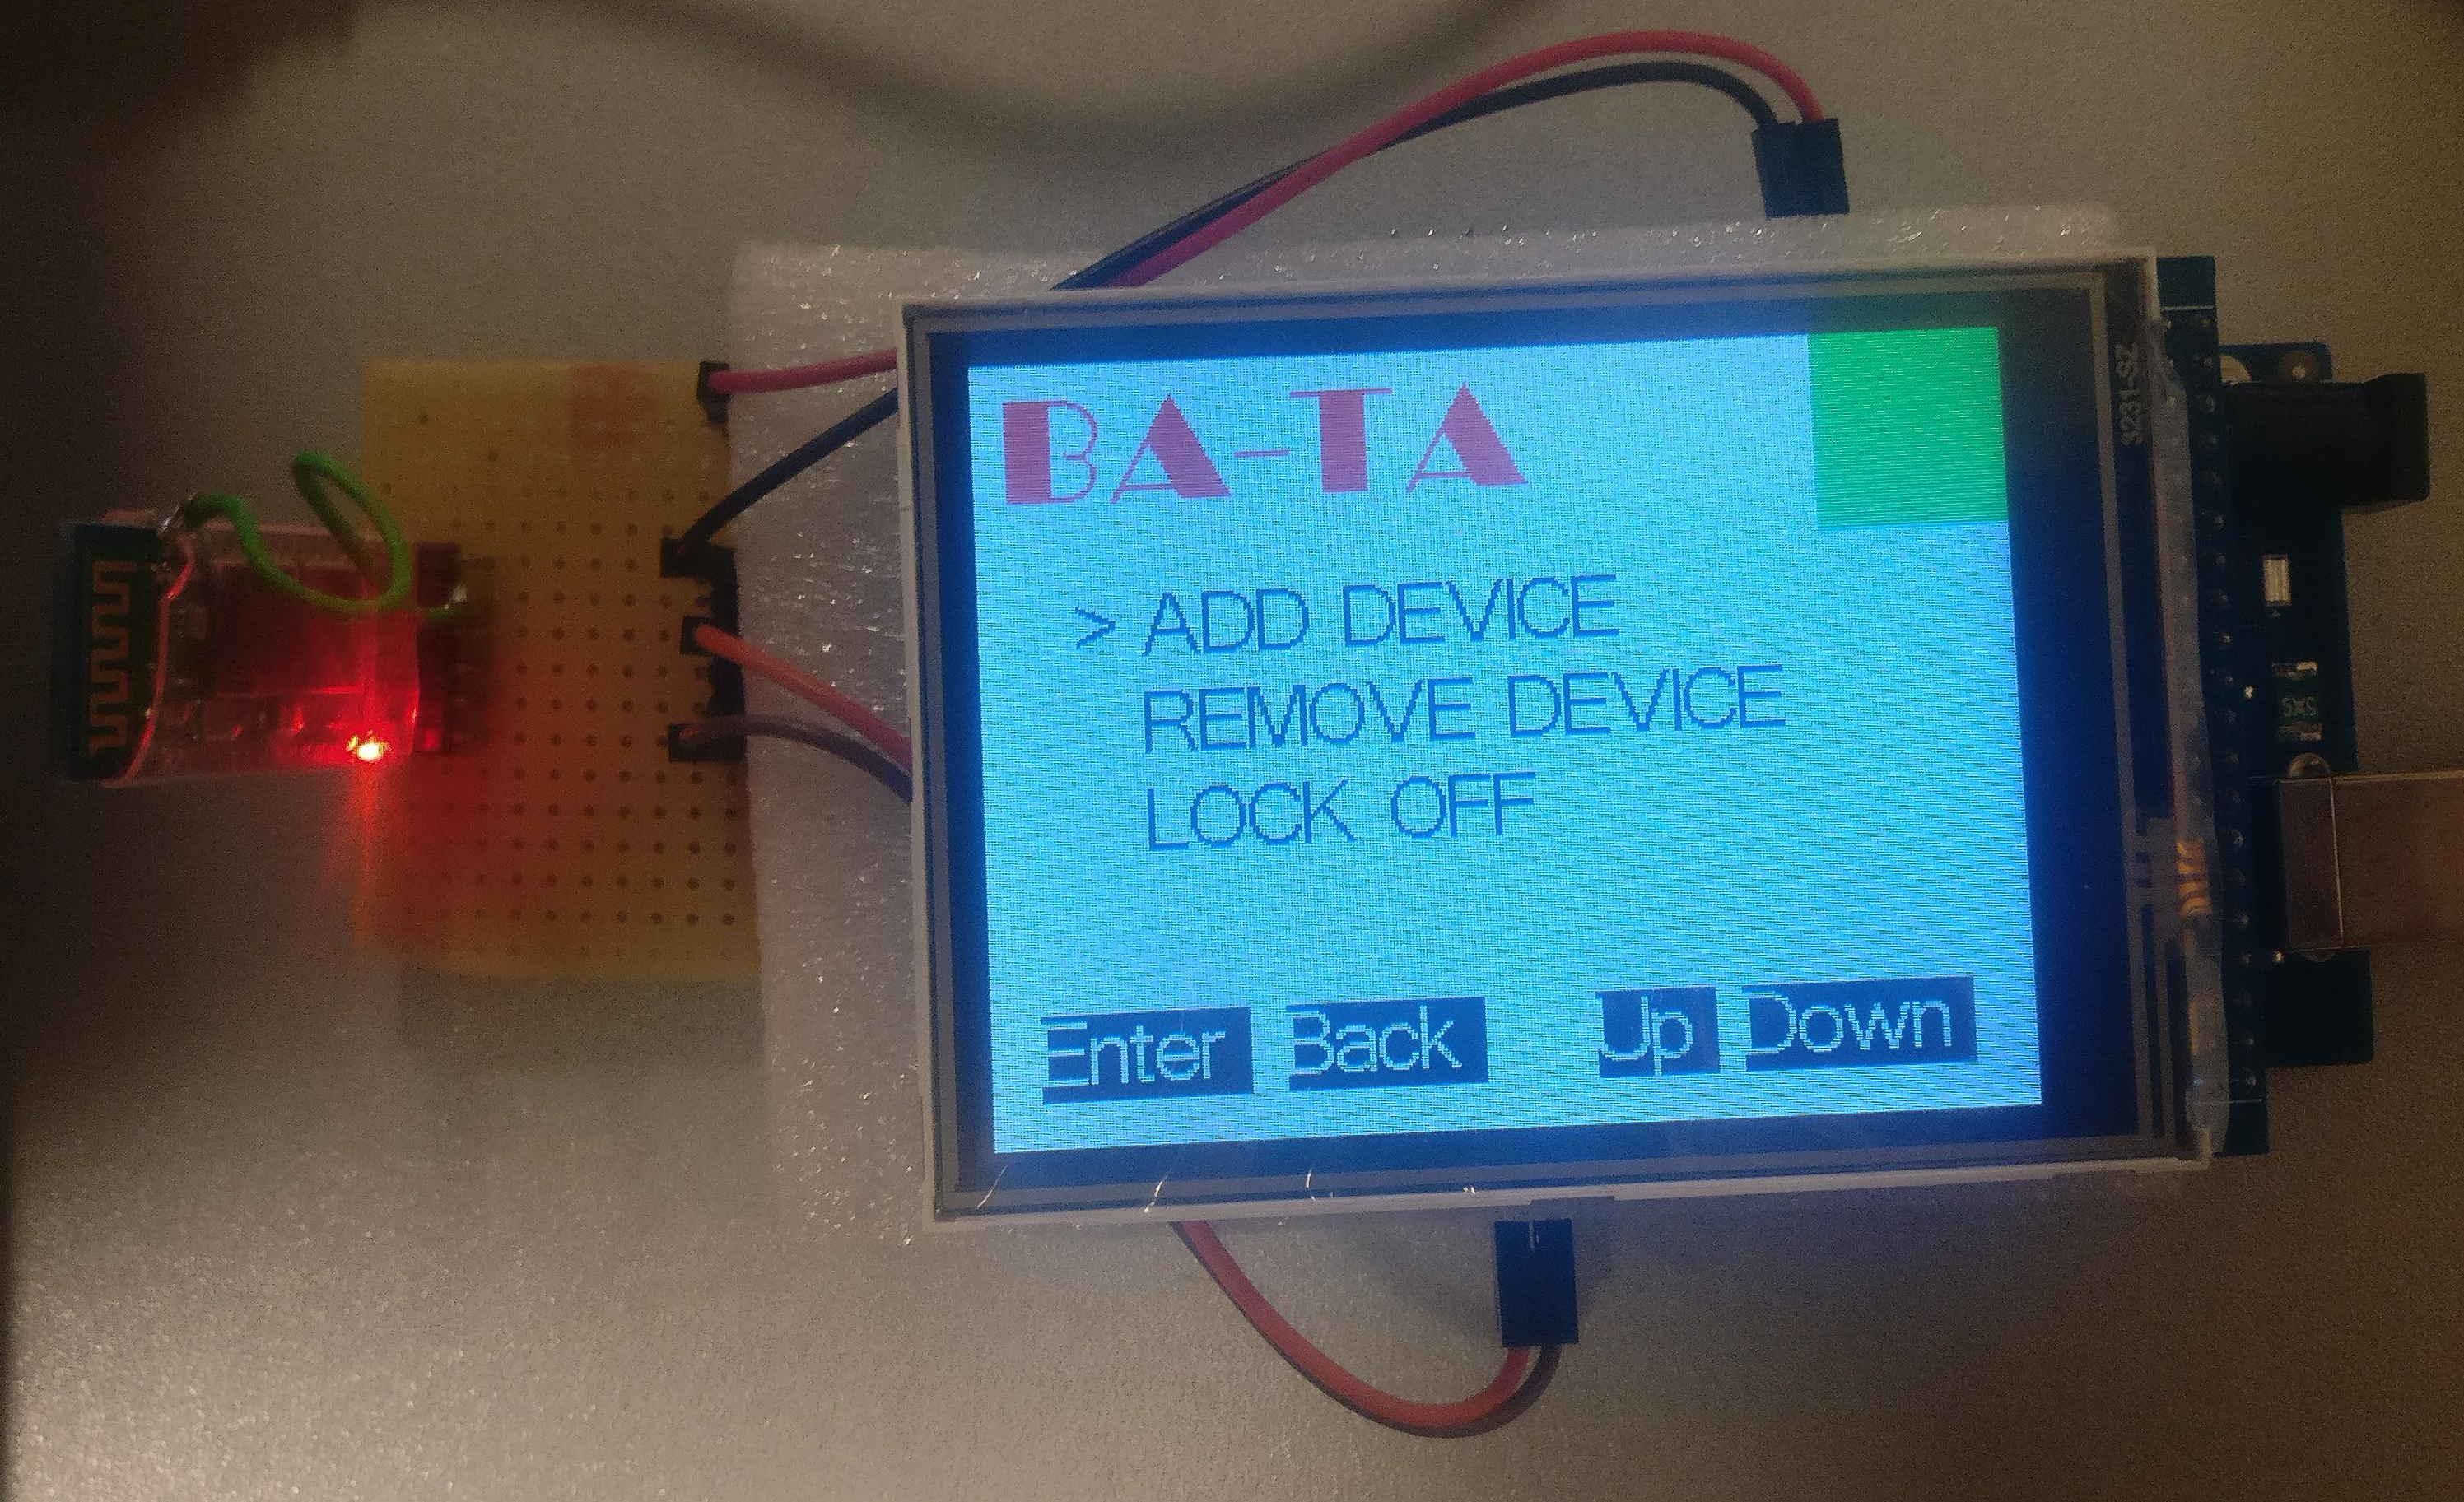
\includegraphics[width = 300 pt]{Img/produkt.png}
	\caption{Prototype af BA-TA}
	\label{fig:prototypeBATA}
\end{figure}